\subsection{Cyclohexanol derivatives}

\subsubsection{Synthesis of the \textit{trans}-2-aminocyclohexan-1-ol head group \compound{cmpd:HOcy6NH2}}

It was decided to produce the cyclohexanol conjugates racemically, with the option of re-synthesising enantiomerically pure versions via the route shown in \ref{sec:HOcy5NH2} if the compounds showed biological activity.

Production of the cyclohexanol conjugates began with the synthesis of \textit{trans}-2-aminocyclohexan-1-ol \compound{cmpd:HOcy6NH2} (see \ref{sch:HOcy6NH2_synth}), using a procedure reported by Xue \textit{et al.}\cite{Xue2006}.
Cyclohexene oxide \compound{cmpd:Ocy6} was opened using ammonia in water and methanol. Initially the reaction was carried out at 85 $^{\circ}$C in a microwave reactor for 30 min, but a large amount of the disubstituted amine could be seen by LCMS (in a ratio of 4:3 product to impurity by NMR). The reaction was therefore attempted at room temperature, and proceeded overnight in high yield and with minimal side reaction.

\begin{scheme}[H]
	\begin{center}
		\schemeref[Ocy6]{cmpd:Ocy6}
		\schemeref[HOcy6NH2]{cmpd:HOcy6NH2}
		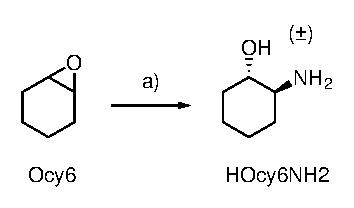
\includegraphics[scale=1]{HOcy6NH2_synth}
		\caption{Synthesis of \textit{trans}-2-aminocyclohexan-1-ol \compound{cmpd:HOcy6NH2}.
		a) \ce{NH3}, water, MeOH, r.t., 72 h, 86\%.
		\label{sch:HOcy6NH2_synth}}
	\end{center}
\end{scheme}

\subsubsection{Synthesis of the \textit{trans}-cyclohexanol- and cyclohexanone-CipMe conjugates \compound{cmpd:HOcy6NH4CipMe} and \compound{cmpd:Ocy6NH4CipMe} \label{sec:Ocy6}}

Carboxylic acid \compound{cmpd:HOO4CipMeTFA} was coupled with \textit{trans}-2-aminocyclohexan-1-ol \compound{cmpd:HOcy6NH2} using standard peptide coupling conditions to give \textit{trans}-cyclohexanol-CipMe conjugate \compound{cmpd:HOcy6NH4CipMe} in 32\% yield.

A portion of the \textit{trans}-cyclohexanol-CipMe conjugate \compound{cmpd:HOcy6NH4CipMe} was then oxidised to the ketone using Dess-Martin periodinane and the product was isolated in good yield.

\begin{scheme}[H]
	\begin{center}
		\schemeref[HOcy6NH2]{cmpd:HOcy6NH2}
		\schemeref[HOO4CipMe]{cmpd:HOO4CipMeTFA}
		\schemeref[HOcy6NH4CipMe]{cmpd:HOcy6NH4CipMe}
		\schemeref[Ocy6NH4CipMe]{cmpd:Ocy6NH4CipMe}
		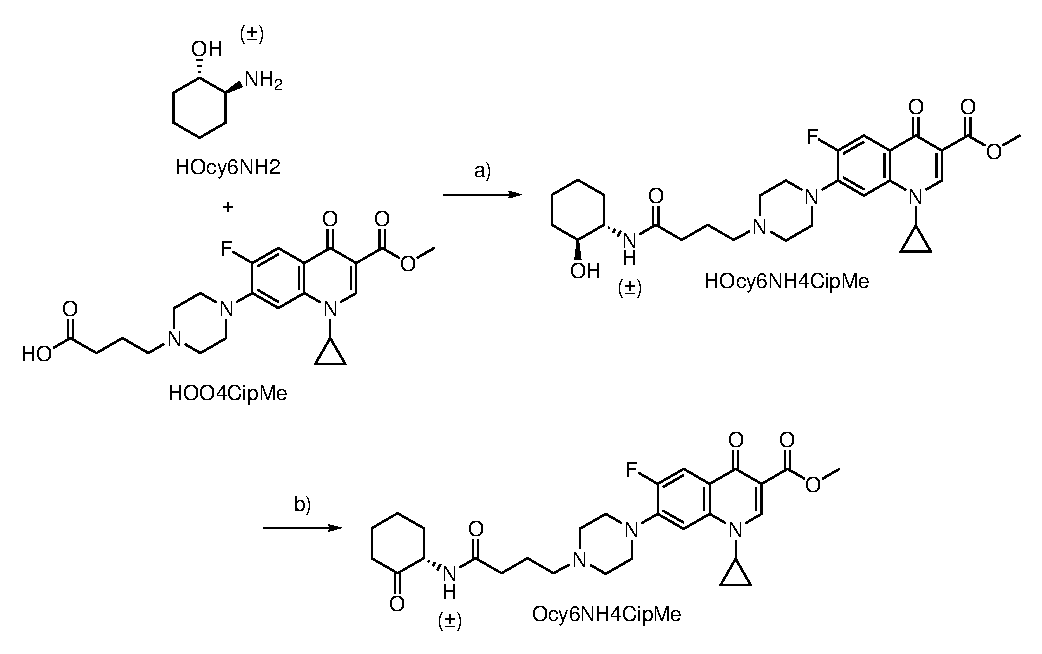
\includegraphics[scale=1]{HOcy6NH4CipMe_synth}
		\caption{Synthesis of the cyclohexanol-CipMe conjugate \compound{cmpd:HOcy6NH4CipMe} and the cyclohexanone-CipMe conjugate \compound{cmpd:Ocy6NH4CipMe}. 
		a) EDC, HOBt, DIPEA, DMF, r.t., 16 h, 32\%.
		b) DMP, \ce{CH2Cl2}, r.t., 6 h, 69\%.
		\label{sch:HOcy6NH4CipMe_synth}}
	\end{center}
\end{scheme}

\subsubsection{Synthesis of the \textit{trans}-cyclohexanol- and cyclohexanone-Cip triazole conjugates \compound{cmpd:HOcy6NH4T4Cip} and \compound{cmpd:Ocy6NH4T4Cip}}

The triazole conjugates were synthesised using the route described in \ref{sec:Cl4Cl}. Cl-C$_4$-\textit{trans}-cyclohexanol \compound{cmpd:HOcy6NH4Cl} was synthesised in good yield from \textit{trans}-2-aminocyclohexan-1-ol \compound{cmpd:HOcy6NH2} and 4-chlorobutyryl chloride \compound{cmpd:Cl4Cl}. 
Cl-C$_4$-\textit{trans}-cyclohexanol \compound{cmpd:HOcy6NH4Cl} was then converted to N$_3$-C$_4$-\textit{trans}-cyclohexanol \compound{cmpd:HOcy6NH4N3} by reaction with sodium azide in excellent yield. 

\begin{scheme}[H]
	\begin{center}
		\schemeref[HOcy6NH2]{cmpd:HOcy6NH2}
		\schemeref[Cl4Cl]{cmpd:Cl4Cl}
		\schemeref[HOcy6NH4Cl]{cmpd:HOcy6NH4Cl}
		\schemeref[HOcy6NH4N3]{cmpd:HOcy6NH4N3}
		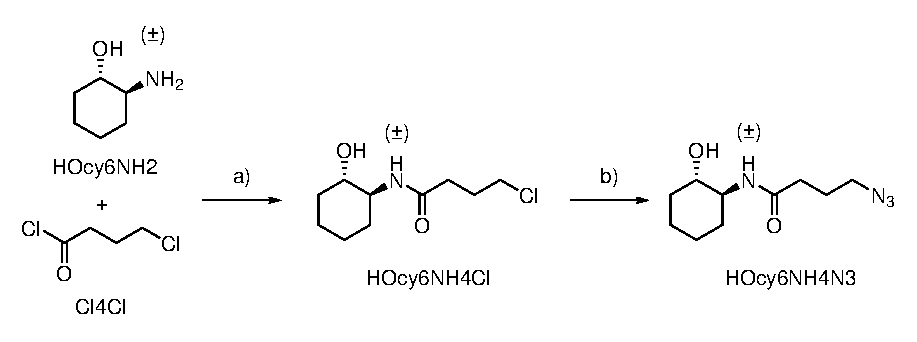
\includegraphics[scale=1]{HOcy6NH4N3_synth}
		\caption{Synthesis of N$_3$-C$_4$-\textit{trans}-cyclohexanol \compound{cmpd:HOcy6NH4N3}. 
		a) TEA, \ce{CH2Cl2}, 0 $^{\circ}$C, 30 min, 76\%.
		b) \ce{NaN3}, acetonitrile, 50 $^\circ$C, 16 h, 98\%.
		\label{sch:HOcy6NH4N3_synth}}
	\end{center}
\end{scheme}

The \textit{trans}-cyclohexanol-Cip triazole conjugate \compound{cmpd:HOcy6NH4T4Cip} was synthesised using standard click conditions (see \ref{sec:click_general}) in 49\% yield.
A portion of the \textit{trans}-cyclohexanol-Cip triazole conjugate \compound{cmpd:HOcy6NH4T4Cip} was then oxidised to the ketone using the same conditions used for the cyclohexanone-CipMe conjugate (see \ref{sec:Ocy6}) in very good yield.

\begin{scheme}[H]
	\begin{center}
		\schemeref[HOcy6NH4N3]{cmpd:HOcy6NH4N3}
		\schemeref[Y4Cip]{cmpd:Y4Cip}
		\schemeref[HOcy6NH4T4Cip]{cmpd:HOcy6NH4T4Cip}
		\schemeref[Ocy6NH4T4Cip]{cmpd:Ocy6NH4T4Cip}
		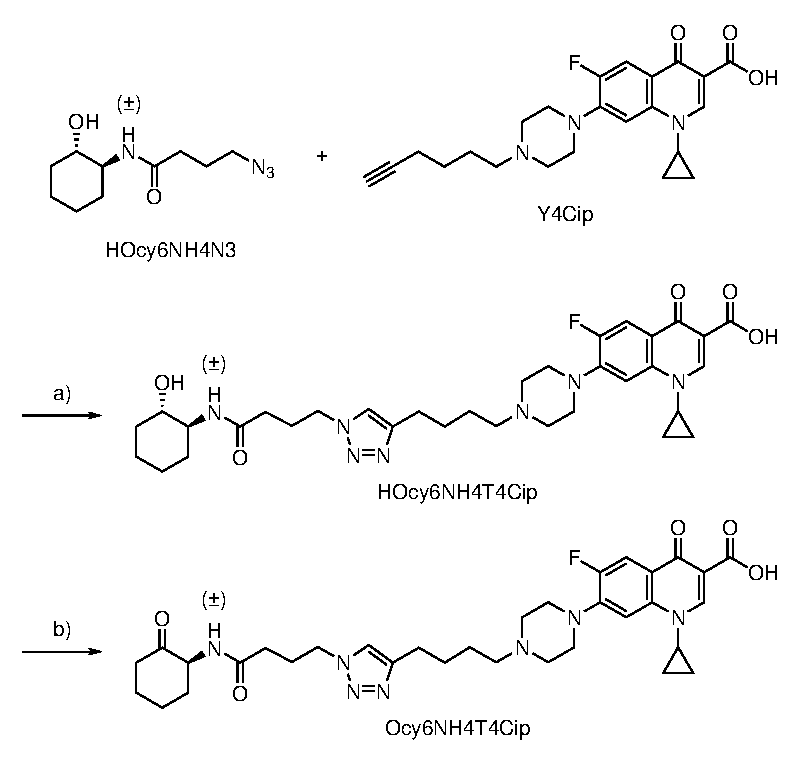
\includegraphics[scale=1]{HOcy6NH4T4Cip_synth}
		\caption{Synthesis of the \textit{trans}-cyclohexanol-Cip triazole conjugate \compound{cmpd:HOcy6NH4T4Cip} and the cyclohexanone-Cip triazole conjugate \compound{cmpd:Ocy6NH4T4Cip}. 
		a) \ce{CuSO4}, THPTA, sodium ascorbate, \ce{H2O}, \textit{t}-BuOH, r.t., 16 h, 49\%. 
		b) DMP, \ce{CH2Cl2}, r.t., 4 h, 78\%.
		\label{sch:HOcy6NH4T4Cip_synth}}
	\end{center}
\end{scheme}